\documentclass{article}
\usepackage{amsmath}
\usepackage{changepage}
\usepackage{float}
\usepackage{amsmath}
\usepackage{tikz}
\usepackage{graphicx}
\usepackage{color}
\usepackage{listings}
\usepackage{color}
\usepackage{algpseudocode}
\definecolor{dkgreen}{rgb}{0,0.6,0}
\definecolor{gray}{rgb}{0.5,0.5,0.5}
\definecolor{mauve}{rgb}{0.58,0,0.82}
\usetikzlibrary{arrows}

\lstset{frame=tb,
  language=Java,
  aboveskip=3mm,
  belowskip=3mm,
  showstringspaces=false,
  columns=flexible,
  basicstyle={\small\ttfamily},
  numbers=none,
  numberstyle=\tiny\color{gray},
  keywordstyle=\color{blue},
  commentstyle=\color{dkgreen},
  stringstyle=\color{mauve},
  breaklines=true,
  breakatwhitespace=true,
  tabsize=3
}

\long\def\/*#1*/{}

\tikzset{
  treenode/.style = {align=center, inner sep=0pt, text centered,
    font=\sffamily},
  1/.style = {treenode, circle, white, font=\sffamily\bfseries, draw=black,
    fill=black, text width=1.5em},% arbre rouge noir, noeud noir
  2/.style = {treenode, circle, white, draw=black, 
    text width=1.5em, very thick},% arbre rouge noir, noeud rouge
  3/.style = {treenode, circle, white, draw=black,
    minimum width=0.5em, minimum height=0.5em}% arbre rouge noir, nil
}
\tikzset{
  treenode/.style = {align=center, inner sep=0pt, text centered,
    font=\sffamily},
  arn_n/.style = {treenode, circle, white, font=\sffamily\bfseries, draw=black,
    fill=black, text width=1.5em},% arbre rouge noir, noeud noir
  arn_r/.style = {treenode, circle, red, draw=red, 
    text width=1.5em, very thick},% arbre rouge noir, noeud rouge
  arn_x/.style = {treenode, rectangle, draw=black,
    minimum width=0.5em, minimum height=0.5em}% arbre rouge noir, nil
}


\begin{document}

\begin{center}
Andreas Bach Landgrebe \\
Computer Science 250: Analysis of Algorithms \\
March 11, 2015 \\
Laboratory Assignment 7 - Sorting Strings  \\
\end{center}
\newpage
\begin{center}
Part One: Parser and Simple Sorting \\
Part Two: Protein Comparison \\
Part Three: New Sorting Algorithms\\
Source Code
\end{center}
\begin{lstlisting}
import java.io.IOException; 
import java.io.*;
import java.util.*;
import java.util.Arrays;
import java.util.Collections;
import java.lang.*;
import java.lang.Object.*;
import java.lang.Number.*;
import java.lang.Integer.*;

public class Lab7 {
    //used mostly for part 1
	public static List<String> identifier = new ArrayList<String>();
	static List<String> sequence = new ArrayList<String>(); 
	static String lineOfFile;
	public static String[] arrayListToArray;
    //used mostly for part 2
	static int [][] a;


	public static void arrayListToArrayConverter(){
		arrayListToArray = new String[identifier.size()];
		for(int i = 0; i < identifier.size(); i++){
			arrayListToArray[i] = identifier.get(i);
		}
	}

	public static void arrayListToArraySequence(){
		arrayListToArray = new String[sequence.size()];
		for(int i = 0; i < sequence.size(); i++) {
			arrayListToArray[i] = sequence.get(i);
		}
	}

	public static String addPeriods(String lineofFile){
			if(lineOfFile.length() < 21){
				while(lineOfFile.length() < 21){
					lineOfFile = lineOfFile + ".";
				} //while
			} //if
			return lineOfFile;
	} //addPeriods methods


	public static void leastCompleteMostComplete(){

       int min = Integer.MAX_VALUE;
       int max = Integer.MIN_VALUE;
       int maxPosition = 0;
       int minPosition = 0;

       for(int i = 0; i < identifier.size(); i++){

            //System.out.println("This identifier: " + identifier.get(i) + " has " + counter(i) + " missing characters");

        if(counter(i) < min){
            min = counter(i);
            minPosition = i;
        }
        if(counter(i) > max){
            max = counter(i);
            maxPosition = i;          
        }
    }
    System.out.println("The max value is: " + max + " was " + identifier.get(maxPosition));
    System.out.println("The min value is: " + min + " was " + identifier.get(minPosition));
}

public static int counter(int value) {
    lineOfFile = sequence.get(value);
    char sequence[] = lineOfFile.toCharArray();
    int missingCharacters = 0;
    for(int i = 0; i < lineOfFile.length(); i++) {
        if(sequence[i] == '-'){
            missingCharacters++;
            } //if
        } //for
        return missingCharacters;
    } //counter method

    public static void parse(File proteinFile) {
        try {

            Scanner scan = new Scanner(proteinFile);

            while(scan.hasNextLine()) {

                lineOfFile = scan.nextLine();

                if(lineOfFile.startsWith(">")) {
                    identifier.add(addPeriods(lineOfFile));
                } else

                if(!lineOfFile.equals("")) {
                    sequence.add(lineOfFile);
            } //if-else
        } //while

        for(int i = 0; i < identifier.size(); i++) {
            System.out.println(identifier.get(i));
            System.out.println(sequence.get(i));
            System.out.println();
            } //for
        } catch (FileNotFoundException e) {
            e.printStackTrace();
        } //try-catch
    //System.out.println("Done");
    } //parse method

/*
    public static int partTwo(){
        int score;
        char[] one;
        char[] two;
        for(int x = 0; a <identifier.size(); i++){
            for (int y = 0; b <identifier.size(); i++){

                lineOfFile = sequence.get(x);
                one[] = lineOfFile.toCharArray();
                lineOfFile = sequence.get(y);
                two[] = lineOfFile.toCharArray();
                for(int z = 0; z < one.length; z++){
                    if(one[z] == '-'){
                    } else 
                    if(one[z] == two[z]) {
                        score = score + 3;
                    } else 
                    if(two[z] == '-') {
                        score = score - 1;
                    } else {
                        score = score - 2;
                    } //if-else
                } //3rd for
            } //two for
        } //one for
        return score;
    }
    */


public static int MostSimilarByIndex(int x, int y) {
        int score = 0;
        lineOfFile = sequence.get(x);
        char one[] = lineOfFile.toCharArray();
        lineOfFile = sequence.get(y);
        char two[] = lineOfFile.toCharArray();
        for(int z = 0; z < one.length; z++) {
            if (one[z]=='-') {
            } else if(one[z]==two[z]) {
                score = score + 3;
            } else if (two[z]=='-') {
                score = score -1;
            } else {
                score = score -2;
            }
        }
        return score;
    }
    //using two dimensional array to pass to the size of the identifier
    public static void score() {
        int size = identifier.size();
        a = new int [size][size];
        for(int x = 0; x < identifier.size(); x++) {
            for(int y = 0; y < identifier.size(); y++) {
                a[x][y] = MostSimilarByIndex(x,y);
            }
        }
    }
    
    public static void maximumMinimumPositionAndValue() {
        int min = Integer.MAX_VALUE;
        int max = Integer.MIN_VALUE;
        int minimumPositionX = 0;
        int minimumPositonY = 0;
        int maximumPositionX = 0;
        int maximumPositionY = 0;
        for(int x = 0; x < identifier.size(); x++) {
            for(int y = 0; y < identifier.size(); y++) {
                if (x == y) {
                } else if(a[x][y] < min) {
                    min = a[x][y];
                    minimumPositionX = x;
                    minimumPositonY = y;
                } else if(a[x][y] > max) {
                    max = a[x][y];
                    maximumPositionX = x;
                    maximumPositionY = y;
                }               
            }
        }
        System.out.println("Maximum score = " + max);
        System.out.println(identifier.get(maximumPositionX)+" vs. "+identifier.get(maximumPositionY));
        System.out.println("Minimum score = " + min);
        System.out.println(identifier.get(minimumPositionX)+" vs. "+identifier.get(minimumPositonY));
    }

    public static void dTIMCore() {
        int locationOfArrayIndex = identifier.size()-1;
        int min = Integer.MAX_VALUE;
        int max = Integer.MIN_VALUE;
        int minPosition = 0;
        int maxPosition = 0;
        double scores = 0.0;
        for(int x = 0; x < identifier.size(); x++) {
            if (x == locationOfArrayIndex) {
            } else if(a[locationOfArrayIndex][x] < min) {
                min = a[locationOfArrayIndex][x];
                minPosition = x;
            } else if(a[locationOfArrayIndex][x] > max) {
                max = a[locationOfArrayIndex][x];
                maxPosition = x;
            } //if-else
            scores = scores + a[locationOfArrayIndex][x];
        }//640
        System.out.println("Maximum score to dTIM_core = " + max);
        System.out.println("Most similar protein: "+identifier.get(maxPosition));
        System.out.println("Minimum score to dTIM_core = " + min);
        System.out.println("Least similar protein: "+identifier.get(minPosition));
        System.out.println("Average Score in the TIM family is: " + scores/640.0);
    }

} //Lab7 class
\end{lstlisting}
\begin{center}
Main File
\end{center}
\begin{lstlisting}
import java.util.*;
import java.io.*;

public class Lab7MainFile {


	public static void main(String[] args) {
		Lab7 sc = new Lab7();
		String proteinFile = "cTIM_core_align.fa";
		File file = new File(proteinFile);
		sc.parse(file);
		sc.leastCompleteMostComplete();
		sc.score();
		sc.maximumMinimumPositionAndValue();
		sc.dTIMCore();
		//sc.arrayListToArrayConverter(); 
		/*
		uncomment top line for running through the identifier
		and comment the bottom line

		uncomment the bottom line for running through the sequence 
		and comment the top line

		dont uncomment both of them, it will not run correctly
		*/
		sc.arrayListToArraySequence();
		
		time("Merge", sc.arrayListToArray);
		double t1 = time("Merge", sc.arrayListToArray);
		double t2 = time("LSD", sc.arrayListToArray);
		double t3 = time("Quick", sc.arrayListToArray);
		double t4 = time("MSD", sc.arrayListToArray);

		String alg1 = "Merge";
		String alg2 = "LSD";
        StdOut.printf("In the file cTIM_core_align.fa\n    %s is", alg1);
        StdOut.printf(" %.3f times faster than %s\n", t2/t1, alg2);       

        String alg3 = "Quick";
        String alg4 = "MSD";

 	    StdOut.printf("In the file cTIM_core_align.fa\n    %s is", alg3);
        StdOut.printf(" %.3f times faster than %s\n", t2/t3, alg2); 

        StdOut.printf("In the file cTIM_core_align.fa\n    %s is", alg1);
        StdOut.printf(" %.3f times faster than %s\n", t4/t1, alg4); 

        StdOut.printf("In the file cTIM_core_align.fa\n    %s is", alg3);
        StdOut.printf(" %.3f times faster than %s\n", t4/t3, alg4); 

        StdOut.printf("In the file cTIM_core_align.fa\n    %s is", alg2);
        StdOut.printf(" %.3f times faster than %s\n", t4/t2, alg4); 
         //StdOut.printf("For %d random Doubles\n    %s is", N, alg1);
         //StdOut.printf(" %.3f times faster than %s\n", t2/t1, alg2);       


	}

	public static double time(String alg, String[] a) {
        Stopwatch timer = new Stopwatch();

        if (alg.equals("Insertion")) {
            Insertion.sort(a);
        } else if (alg.equals("Selection")) {
            Selection.sort(a);
        } else if (alg.equals("Shell")) {
            Shell.sort(a);
        } else if (alg.equals("Merge")) {
            Merge.sort(a);
        } else if (alg.equals("Quick")) {
            Quick.sort(a);
        } else if (alg.equals("Heap")) {
            Heap.sort(a);
        } else if (alg.equals("LSD")) {
            LSD.sort(a, 21);
        } else if (alg.equals("MSD")) {
            MSD.sort(a);
        }//if-else
        return timer.elapsedTime();
    } //time
} //Lab7MainFile class
\end{lstlisting}
\begin{center}
Answers to Part One \& Part Two Questions \\
\end{center}
\noindent
Part One
\begin{enumerate}
\item Which protein sequence is the most complete (fewest "-" characters? Which is the least complete? Give the protein identifiers.
\\
Protein Identifier for most complete: $>TPIS_ASPOR/5-247$
\\
\\
Protein Identifier for least complete: $>Q8ISS5_9NEOP/1-23$
\\
\item How many amino acids are missing for the most complete sequence? How many are missing from the least complete sequence?
\\
Number of amino acids that are missing from the most complete sequence: 0
\\
\\
Number of amino acids that are missing from the least complete sequence: 217
\end{enumerate}
\noindent
Part Two
\begin{enumerate}
\item Which protein sequence is the most similar to $dTIM_core$? Which is the least similar? Again, give the protein identifiers.
\\
Most Similar Protein Sequence: $>Q7PXW5_ANOGA/21-259$
\\
\\
Least Similar Protein Sequence: $>TPIS_HALN1/1-207$
\\
\item What was the most similarity score for the most similar sequence? What about the least similar sequence? What was the average similarity score in the TIM family?
\\
\\
Most Similarity Score: 387
\\
\\
Least Similarity Score: -220
\\
\\
Average Similarity Score: 81.3765625
\end{enumerate}
\begin{center}
Part 3: New Sorting Algorithm
\end{center}
\begin{center}
\begin{figure}[H]
\begin{tabular}{| l | l | l | l | l | l | l | l |}
\hline
Identifier & Run 1 & Run 2 & Run 3 & Run 4 & Run 5 & Mean(Average) & Standard Devitation\\ \hline
Merge vs LSD & 2 & 1 & 1  & 1 & 2 & 1.4 & 0.48989794855664 \\ \hline
Quick vs LSD & 0.333 & 0.333 & 0.4  & 0.5 & 0.6 & 0.4332 & 0.10340870369558 \\ \hline
Merge vs MSD & 7 & 5 & 5 & 5 & 6 & 5.6 & 0.8\\ \hline
Quick vs MSD& 1.833 & 1.667 & 1.4  & 2.5 & 1.2 & 1.72 & 0.44649255312939\\ \hline
LSD vs MSD & 3.5 & 3 & 3.5 & 3 & 2 & 3 & 0.54772255750517\\ \hline
\end{tabular}
\caption{Results from Running  different Algorithms for Iterative Array Values}

\end{figure}
\end{center}
\begin{center}
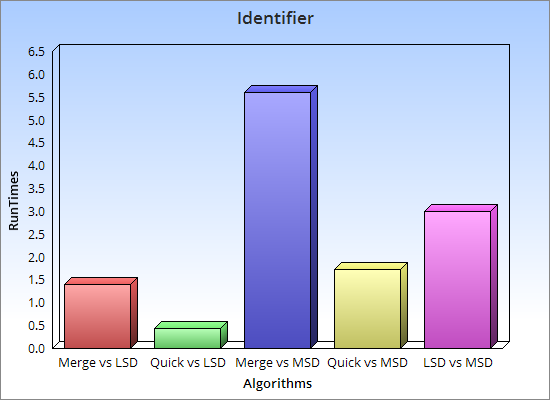
\includegraphics[scale=0.6]{Identifier.png}
\end{center}
\begin{center}
\begin{figure}[H]
\begin{tabular}{| l | l | l | l | l | l | l | l |}
\hline
Sequence & Run 1 & Run 2 & Run 3 & Run 4 & Run 5 & Mean(Average) & Standard Devitation\\ \hline
Merge vs LSD & 3 & 1 & 1  & 2 & 1.5 & 1.7 & 0.74833147735479 \\ \hline
Quick vs LSD & 0.6 & 0.333 & 0.333  & 0.5 & 0.375 & 0.4282 & 0.10547682209851 \\ \hline
Merge vs MSD & 32.5 & 31.5 & 32.5 & 36 & 33.5 & 33.2 & 1.5362291495737\\ \hline
Quick vs MSD & 11.4 & 10.5 & 10.833 & 9 & 11.167 & 10.58 & 0.84661419784929 \\ \hline
LSD vs MSD & 30.5 & 31.5 & 32.5 & 33 & 33.5 & 32.2 & 1.0770329614269\\ \hline
\end{tabular}
\caption{Results from Running  different Algorithms for Sequence Array Values}
\end{figure}
\end{center}
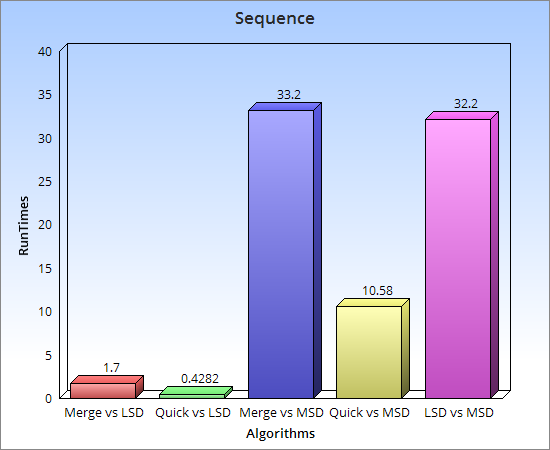
\includegraphics[scale=0.6]{Sequence.png}
\newpage
\begin{center}
Part Four: While You Have Some Downtime
\end{center}
\begin{enumerate}
\item Give a trace of LSD String Sort for this set of keys: BCA, ABC, ABA, CAA, CBA, BAC, CAB, BCA, CBA
\tikzstyle{block} = [rectangle, draw, fill=blue!20, 
    text width=6em, text centered, rounded corners, minimum height=6em]
\tikzstyle{line} = [draw, -latex']
    
\begin{tikzpicture}[node distance = 2cm, auto]
    % Place nodes
     \node [block] (first) {BCA\\
ABC\\
ABA\\
CAA\\
CBA\\
BAC\\
CAB\\
BCA\\
CBA\\
input (w  = 3)};
    \node [block, right of=first, node distance = 2.9cm](second) {
BCA\\
ABA\\
CAA\\
CBA\\
BCA\\
CBA\\
CAB\\
ABC\\
BAC\\
d = 2  
        };
            \node [block, right of=second, node distance = 2.9cm](third) {
CAA\\
CAB\\
BAC\\
ABA\\
CBA\\
CBA\\
ABC\\
BCA\\
BCA\\
d = 1  
        };
            \node [block, right of=third, node distance = 2.9cm](fourth) {
ABA\\
ABC\\
BAC\\
BCA\\
BCA\\
CAA\\
CAB\\
CBA\\
CBA\\
d = 0
};
\node [block, right of=fourth, node distance = 2.9cm](fifth) {
ABA\\
ABC\\
BAC\\
BCA\\
BCA\\
CAA\\
CAB\\
CBA\\
CBA\\
output
};
    % Draw edges
    \path [line] (first) -- (second);
	\path [line](second) -- (third);
	\path [line](third) -- (fourth);
	\path [line](fourth) -- (fifth);
    
\end{tikzpicture}
\newpage
\item Give a trace of MSD String Sort for this set of keys: A, AAAA, AA, AAB, AAA, ABA, BAAAAA
\begin{lstlisting}
A
AAAA
AA
AAB
AAA
ABA
BAAAAA
\end{lstlisting}
\textbf{A \\
AAAA \\
AA\\
AAB\\
AAA\\
ABA} \\
BAAAAA
\\
\\
A \\
\textbf{AAAA \\
AA \\
AAB \\
AAA \\
ABA} \\
BAAAAA \\
\\
\\

A \\
AA \\
\textbf{AAAA \\
AAA\\
AAB} \\
ABA \\
BAAAAA \\
\\
\textbf{RESULTS }
\\
A\\
AA\\
AAAA\\
AAA\\
AAB\\
ABA\\
BAAAAA\\
\newpage
\item We noted in the lecture that the \~{} 7WN + 3WR runtime for LSD String Sort simplifies to being proportional to \~{} 7WN when N is a much larger value than R. Assuming an alphabet of 256 characters and an average string length of 10 characters, what is the smallest value of N required for this approximation to be within 1\% of the original computation?
\\
$\frac{7wn}{7wn + 3wr} >= \frac{99}{100}$\\
$700N >= 99 (7N +3R)$\\
$N = 10, 862$
\end{enumerate}




\end{document}